% !TEX root = main.tex

%%%%%%%%%%%%%%%%%%%%%%%%%%%%%%%%%%%%%%%%%%%%%%%%%%%%%%%%%%%%%%%%%%%%%%%%%%%%%%%%
\chapter{Introduction}

The 3D scanning of outdoor structures gained a lot of interest recently. The emergence of cheap and easy-to-use 3D sensors brought its share of new applications, enabling the digitization of the world by the masses. Most of common everyday 3D scanning devices are captive of the indoors, though. There is yet to find a way to give everyone the chance to scan building-scale objects, bridging the gap between indoor and outdoor scanning.

This thesis proposes to do so simply by using cameras, and an existing reconstruction technique dubbed ``Photometric Stereo'' (PS). The idea is to point a camera towards a scene to be scanned, and to capture a time-lapse sequence over time. Variations in the illumination conditions can be used by PS to reconstruct the shape of the observed scene. PS has been known in computer vision for more than 35 years, and is still an active area of research. It is an excellent choice for shape reconstruction given its great output density and stellar results in laboratory conditions.

\section{Photometric Stereo}
\label{sec:ps_ori}

The first definition of PS, made in 1979 by Woodham~\cite{Woodham1979}, made a lot of assumptions to simplify the problem to its essence, such as these ones:
\todo{inline}
\begin{itemize} \setlength\itemsep{-0.2em}
  \item The object surface reflectance must be
  \vspace{-0.65em}\begin{itemize} \setlength\itemsep{0.1em}
    \item Lambertian;
    \item constant;
  \end{itemize} \vspace{-0.4em}
  \item The object is rigid (normals are constant over time);
  \item Lighting is known;
  \item Lighting is a distant point light source;
  \item Sensors are noiseless;
  \item All the images are aligned.
\end{itemize}
In its essence, everything must be constant; only the illumination should vary over the sequence.

Following these assumptions, the Lambertian image formation model for a single pixel is defined as
\begin{equation}
b_t =  \rho \; \mathbf{l} \mathbf{n}_t \quad,
\end{equation}
where pixel $t$ will have an intensity $b_t$ when the corresponding surface patch normal $\mathbf{n}_t$ of albedo $\rho$ is lit by a point light source with an incident vector $\mathbf{l}$. For the sake of simplification, its albedo. Likewise, the incident lighting vector $\mathbf{l}$ is scaled by its intensity.

This means that the appearance of a pixel in an image, with the aforementioned assumptions, is dependent on 1) the normal and albedo of a visible surface patch, and 2) the incident angle and intensity of the light. Woodham realized that if a pixel appearance depends on the surface normal, it meant that this surface normal can be found from a known pixel appearance. This means that the shape of an object (through its surface normals) could be obtained by observing the pixels appearance. But there's a problem: a single pixel intensity cannot explain all three degrees of freedom of the normal to be reconstructed (scaled by its albedo), leading to an underconstrained problem.

To solve this issue, it is possible to take a sequence of images, all from the same viewpoint, but with different lighting conditions. The shading difference between the different lighting conditions can constrain the problem correctly. In the case of a sequence of images, we define $\mathbf{L}$ as the stacked incident vectors of all the $m$ images in the sequence (labeled $\mathbf{l}_{1}, \mathbf{l}_{2}, \dots \mathbf{l}_{m}$):
\begin{equation}
\mathbf{L} =
\begin{bmatrix}
    \mathbf{l}_{1} \\
    \mathbf{l}_{2} \\
    \vdots \\
    \mathbf{l}_{m}
\end{bmatrix}
\quad,
\end{equation}
which can be used to define the appearance of all pixels over all the images of the sequence, as such:
\begin{equation}
\label{eq:lamb_refl}
\mathbf{b} =  \rho \mathbf{L} \mathbf{n} \quad.
\end{equation}

Solving eq.~\eqref{eq:lamb_refl} for $\mathbf{n}$ gives the relation
\begin{equation}
\label{eq:original_form}
\rho \mathbf{n} =  \mathbf{L}^{-1} \mathbf{b} \quad,
\end{equation}
giving birth to the Photometric Stereo technique.

$\mathbf{n}$ provides the structure of the scene visible in the image sequence, giving a single normal for each pixel of the image. This output is called a normal map, because it maps a surface normal to each surface patch visible by a pixel. Integrating this normal map results in an height map (also called depth map), which represents the height of the surface at each sample point. To summarize, PS outputs a normal map, the gradient of the height map.

A concrete example of PS can be seen in fig.~\ref{fig:PS_example}, where a sequence of images and its lighting directions are set as inputs of eq.~\eqref{eq:original_form} to give a normal map in output and its integrated surface, shown in fig.~\ref{fig:PS_example_res}.

The great strength of this technique is its output density: 3D information will be generated for every pixel of one input image. This means that a sequence of 5 megapixels images, as can be found on many current off-the-shelf cameras and cellphones, will generate an output of 5 million 3D points using PS. This quantity of information is impressive given the cost of point and shoot cameras and the ubiquity of cellphones.

Even with all the assumption we made, one issue remains: the lighting directions over the sequence must not be coplanar. If they are coplanar, eq.~\ref{eq:original_form} will result in an underconstrained system, leaving an unknown degree of freedom. This led Woodham to believe that PS ``does not apply to outdoor images taken at different times during the same day [...] since the sun's path across the sky is planar''.

%\begin{equation}
%\mathbf{b} = \rho L(\mathbf{\boldomega}) \langle \boldomega, {\bf n} \rangle \,,
%\end{equation}

\begin{figure}
\centering
%\begin{tabular}{cccccc|ccc}

\includegraphics[width=.15\linewidth]{PS/cat_0.png}

\includegraphics[width=.15\linewidth]{PS/cat_3.png}

\includegraphics[width=.15\linewidth]{PS/cat_4.png}

\includegraphics[width=.15\linewidth]{PS/cat_5.png}

\includegraphics[width=.15\linewidth]{PS/cat_10.png}

\includegraphics[width=.15\linewidth]{PS/cat_11.png}
%
\includegraphics[width=.08\linewidth]{PS/cat_normal_map.png}
%
\includegraphics[width=.04\linewidth]{PS/sphere_nm.png}
%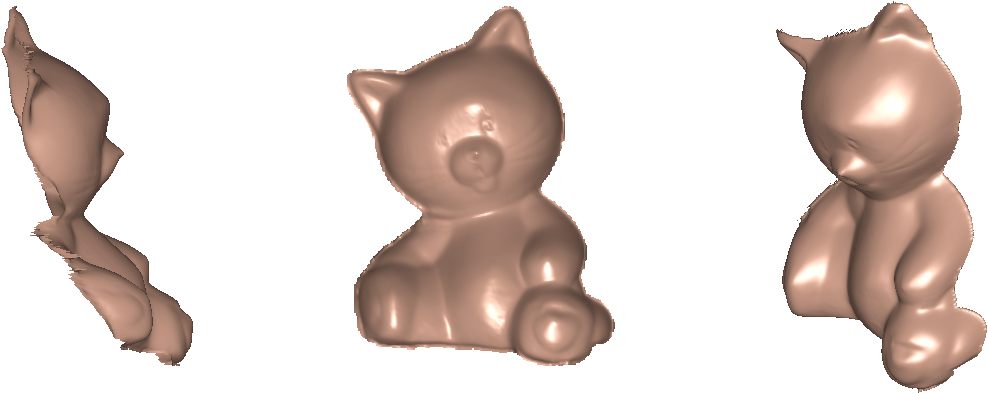
\includegraphics[width=.18\linewidth]{PS/3d.png}
%a) & b) & c) & d) & e) & f) & g) & h) & i)
%\end{tabular}
\caption{Examples of inputs lit from different directions, g) normal map obtained from the original form of the Photometric Stereo algorithm, h) sphere normal map showed as example, i) reconstructed surface from 3 viewpoints.\newline
{\small input images from CSE 455, 2010 by Neel Joshi, Ira Kemelmacher and Ian Simon}
}
\label{fig:PS_example}
\end{figure}

\begin{figure}
\begin{tabular}{ccc}

\includegraphics[height=3.8cm]{PS/cat_normal_map.png} &

\includegraphics[width=.15\linewidth]{PS/sphere_nm.png} &
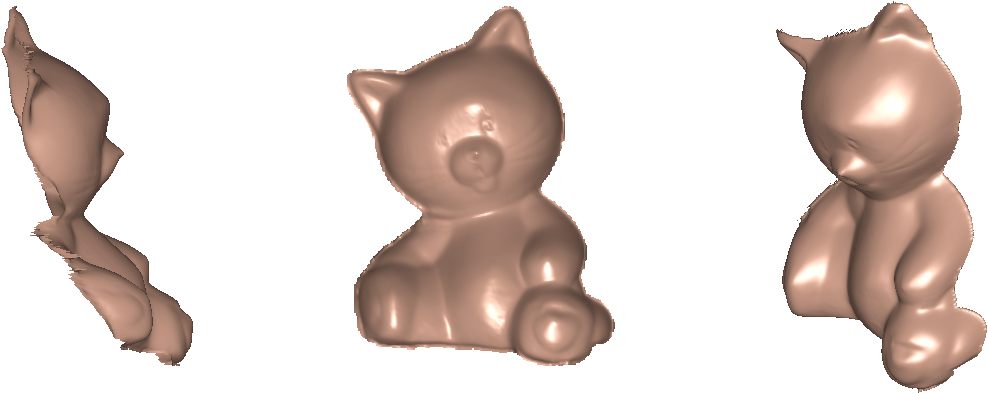
\includegraphics[height=3.8cm]{PS/3d.png} \\
(a) & (b) & (c)
\end{tabular}
\caption{Results from the inputs in \ref{fig:PS_example}. (a) normal map obtained from the original form of the Photometric Stereo algorithm, (b)) sphere normal map showed as example, (c)) reconstructed surface from 3 viewpoints.}
\label{fig:PS_example_res}
\end{figure}

\section{Outdoor Photometric Stereo}

A lot of work have been done on PS since its original definition. Contrary to what Woodham believed, PS has recently been applied to outdoor photographs, mainly images captures by outdoor cameras. Unfortunately, outdoor lighting is complex and uncontrollable, therefore the techniques proposed in this domain require capturing either months of data, or the illumination conditions at each frame, none of which is a very practical scenario for the casual user.

To make PS work outdoor, the traditionally employed approximation models such as directional lighting will be replaced by a new data-driven model of natural illumination learned from a large database of high quality sky photographs. This database will be captured over extended periods of time, and will contain thousands of photos of the sky in different illumination conditions. By observing the sky directly, the data-driven model will accurately capture what the likely natural illumination conditions are for a given scene. This enhanced lighting model will better constrain the PS optimization algorithm, allowing it to converge toward real or plausible sky illumination conditions. The resulting shape estimation will better explain the observed input images, giving increased result quality. The key to bring PS outdoor is to understand natural illumination.

\section{Thesis proposal}

The main goal of this thesis is to \textbf{understand how natural illumination impacts PS, effectively tying the reconstruction performance to the sky appearance}. This leads to multiple applications, such as large-scale outdoor scenes reconstruction from short time intervals, without the need for capturing the lighting conditions.

In this thesis, I propose to:
\begin{enumerate}
  \item bring a deeper understanding of the way PS can work outdoors;
  \item introduce a practical PS reconstruction algorithm in the calibrated case;
  \item introduce a practical PS reconstruction algorithm in the uncalibrated case;
\end{enumerate}
These objectives can be attained by a better comprehension of natural illumination and its impact on shading. This knowledge can then be leveraged to improve existing reconstruction algorithms or make new ones that works with complex and uncontrolled lighting conditions.

This thesis will bring answers to questions like:
\begin{itemize}
  \item What is the minimum timelapse interval required to perform PS outside?
  \item What sky characteristics are tied to PS reconstruction performance?
  \item How can we reconstruct an object with natural illumination using PS?
  \item What is the optimal input for PS when considering a 24h interval?
\end{itemize}

\section{Anticipated impact}

3D scanning has become a part of everyday life, with sensors such as the Kinect now in everyone's home, effectively bringing 3D scanning capabilities to the masses. Taking the Kinect as example, a plethora of new use cases emerged since its original endeavor to revitalize the entertainment industry. For instance, the 3D printing market that grew significantly over the past few years, brought a new need for scans of household objects. Augmented reality is another avenue that requires a lot of models of real world objects. These are but a tiny fraction of the applications of real world scanning.

While the Kinect enabled myriads of applications in indoor environments, using such sensors outdoors is close to impossible. These kind of sensors are so-called active sensors, meaning that they interact with the scene to work. This usually means projecting light in the scene and sensing it back. But this method is problematic outside: the light patterns they emit are completely drowned by the sunlight. In outdoor settings, the only current possibility is to use very expensive scanners, out of reach for the casual user due to their complexity and operational cost. The idea is to bring back the availability and cheapness of sensors such as the Kinect to the outside world.

The level of understanding I propose in this thesis would allow the design and implementation a 3D shape acquisition system that relies only on off-the-shelf cameras, capable of bringing high quality digitization capabilities to anyone with a camera, thus enabling the collaborative reconstruction of large scale outdoor environments. This has the potential of impacting many fields, such as the digital preservation of cultural heritage before it gets damaged by wars, natural disasters, or the passage of time; the replication of real environments in virtual scenarios for the training of first responders or to improve urban planning; the creation of novel, realistic environments for use in video games or special effects in the movie industry; etc. By making these tasks easier, I believe this project will have significant impact on 3D shape acquisition as a whole.